В данной работе расширяющаяся сверхновая аппроксимируется расширяющимся кружком с заданным симметричным профилем поверхностной яркости. Как можно получить значение обусловленной микролинзированием вариации блеска в фиксированный момент времени, то есть для заданного радиуса кружка? Известна следующая формула: наблюдаемый поток $F_{\lambda}(\lambda,t)$ от источника на длине волны $\lambda$ и в момент времени $t$ получается в результате свёртки зависящей от времени яркости кружка-сверхновой $I_{\lambda}(P,\phi,\lambda, t)$ с "накрываемым" \ им участком усилений карты микролинзирования $\mu(P,\phi)$ в плоскости, перпендикулярной к лучу зрения (\cite{goldstein2018}, \cite{hubersuyu2019}). Так как модель сферически-симметричная, получается, что

\begin{equation}\label{eq:eft}
F_{\lambda}(\lambda,t) = D_L^{-2} \int_0^{2\pi} \int_0^{P_m} I_{\lambda}(P,\phi,\lambda, t) \mu(P,\phi)P dP d\phi,
\end{equation}

\noindent где $\phi$ и $P$ являются азимутальным и прицельным параметрами (полярными координатами точек), $D_L$ - болометрическое расстояние\footnote{Оно связано с расстоянием углового диаметра $D_A$ следующим образом: $D_L = (1+z)^2 D_A$ (\cite{distance_measures}).} (\textit{luminosity distance}) до сверхновой, $P_m$ - максимальный прицельный параметр. Формула \eqref{eq:eft} проиллюстрирована на Рисунке \ref{fig:goldsteinn}. 

\begin{figure}
    \centering
	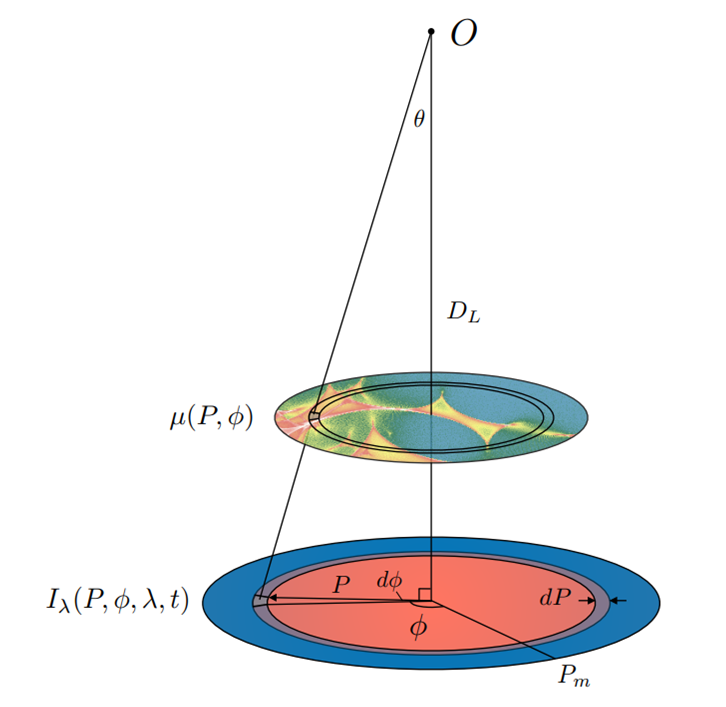
\includegraphics[scale=0.77]{microlensing/images/goldstein.png}
	\caption{Иллюстрация свертки источника с картой (\cite{goldstein2018})} 
	 \label{fig:goldsteinn}
\end{figure}

Сверхновая моделировалась кругом, который расширяется со скоростью $v=500$ км/с в течение 160 дней (в её системе отсчёта). Выбор такого значения скорости обусловлен результатами, полученными при моделировании радиуса фотосферы SN Refsdal (\cite{petrnat2020}). График зависимости радиуса фотосферы от времени приведен на Рисунке \ref{fig:snexpand}.

\begin{figure}[H]
    \centering
	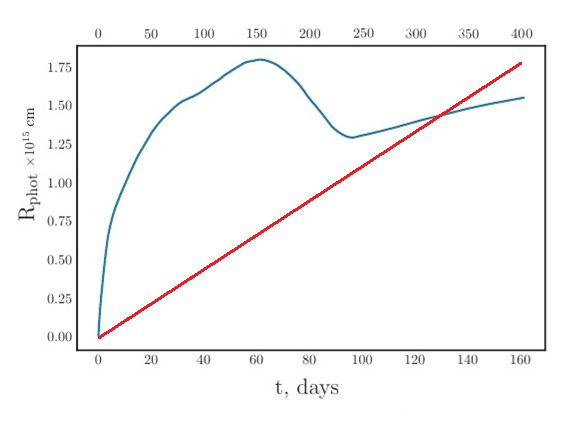
\includegraphics[width=0.8\textwidth]{microlensing/images/snexpand.png}
	\caption{Синий цвет: эволюция радиуса фотосферы $R_{phot}$ в модельном расчёте вспышки сверхновой (\cite{petrnat2020}). Красный цвет: аппроксимация, принятая в данной работе. По горизонтальной оси отложены две временные шкалы: в системе отсчёта сверхновой (снизу) и в системе отсчёта наблюдателя (сверху). Эти шкалы связаны друг с другом множителем $(1+z_{s})\approx 2.5$.}
	\label{fig:snexpand}
\end{figure}

\newpage

Значение абсолютного усиления получается делением потока от кружка-сверхновой, свёрнутого с картой усилений, на значение потока при отсутствии микролинзирования (формула \ref{eq:eft} с $\mu(P,\phi)=1$). Вклад в кривую блеска, обусловленный только микролинзированием, выраженный в звёздных величинах, задаётся выражением:

\begin{equation}\label{eq:deltam}
\Delta m (t)= - 2.5\log \Big[ \frac{L(t)}{S(t)} \Big],
\end{equation}

\begin{equation}\label{eq:iott}
\textrm{где} \ L(t) = \int_0^{2\pi} \int_0^{P_m} I_{\lambda}(P,\phi,\lambda, t) \mu(P,\phi)P dP d\phi
\end{equation}

\begin{equation}\label{eq:sott}
\textrm{и} \ S(t) = \int_0^{2\pi} \int_0^{P_m} I_{\lambda}(P,\phi,\lambda, t) P dP d\phi.
\end{equation}


\noindent Из этой же формулы видно, что в отсутствие микролинзирования $\Delta m =0$. При этом ожидается, что $\Delta m \rightarrow 0$ при $t \rightarrow \infty$, то есть, что большие источники нечувствительны к флуктуациям от микролинзирования.

В рамках моделирования реалистичного профиля яркости сверхновой интенсивность излучения вдоль радиуса аналитически задавалась следующим образом:

\begin{equation}\label{eq:profile}
I(r,t) \propto \frac{1}{2\pi\sigma(t)}\exp\big({\frac{r^2}{2\sigma^2(t)}}\big),
\end{equation}

\noindent где $\sigma(t)$ растёт со временем. Полученные зависимости для 38, 80, 118 и 157 дня с момента взрыва (в системе отсчёта, связанной со сверхновой) приведены на Рисунке \ref{fig:profile}. %Форма (А) аналитически задаётся (б) подробно оописывает профиль яркости

\begin{figure}[H]
    \centering
	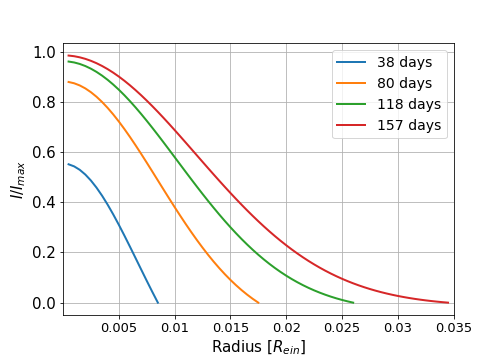
\includegraphics[width=0.8\textwidth]{microlensing/images/profile.png}
	\caption{Нормированный профиль яркости сверхновой в зависимости от радиуса и времени (в системе отсчёта сверхновой) с момента её взрыва ($R_{ein}\approx4.6\cdot10^{14}$ м).}
	\label{fig:profile}
\end{figure}

На Рисунке \ref{fig:example} приведены примеры флуктуации от микролинзирования, рассчитанные по формуле \eqref{eq:deltam}. В одном положении источник при расширении захватывает области сильного усиления, что может заметно повлиять на форму истинной кривой блеска источника (флуктуации $\sim 1$ зв. вел.). В другом положении источник находится в области с практически равномерным усилением и не пересекает каустики; эффект от микролинзирования слабый и примерно постоянный во времени. В каждом положении сверхновая моделировалась диском с плоской засветкой и с гауссовым профилем яркости. Из рисунка можно заключить, что учёт реалистичного распределения яркости сглаживает сильные флуктуации от микролинзирования.

\begin{figure}[H]
    \centering
	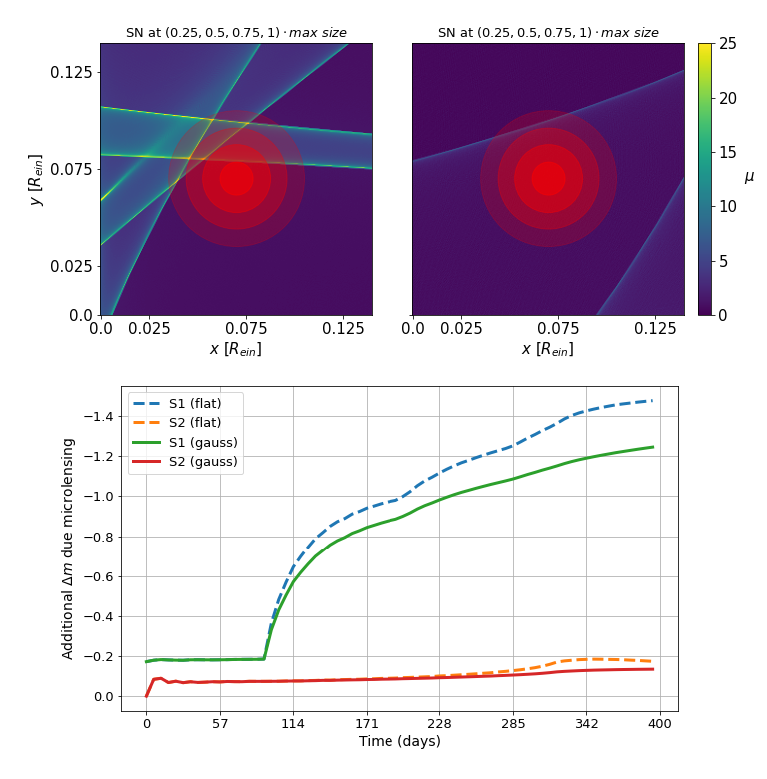
\includegraphics[width=0.99\textwidth]{microlensing/images/caustic.png}
	\caption{\textit{Сверху}: случайные положения сверхновой в изображении S1 (слева) и S2 (справа). \textit{Снизу}: соответствующие этим положениям флуктуации от микролинзирования для источника с плоской засветкой (\textit{flat}) и гауссовым профилем яркости (\textit{gauss}).} 
	\label{fig:example}
\end{figure}

Для статистического анализа микролинзирования был выбран следующий алгоритм. На каждой из карт, изображенных на Рисунке \ref{fig:mymaps}, случайным образом выбираются 50 точек, соответствующих центру расширяющейся сверхновой. Для каждого положения по формуле \eqref{eq:deltam} вычисляются флуктуации микролинзирования и для плоского источника, и для источника с гауссовым профилем яркости. После этого полученные значения прибавляются к кривым блеска SN Refsdal.

%Положения 50 источников на обеих картах и соответствующие им флуктуации приведены на Рисунках \ref{fig:s1} и \ref{fig:s2}.



